%! Author = alexis
%! Date = 20/06/2022

\chapter{Historical Network Analysis and Visualization}\label{ch:related-work}

Social historians rely on textual historical documents to draw socio-economic conclusions about the past.
They read and analyze the documents they can find from a period and subject of interest, and make their conclusions after analyzing them and cross-referencing the information they found.
Several methods have been developed in History to extract and analyze the information contained in the documents in a rigorous way, such as qualitative analysis, quantitative methods, or Historical Social Network Analysis (HSNA).
HSNA is a method coming from Sociology consisting in modeling the relational information mentioned in the documents---such as family, business, or friendship ties---in a network, to be able to characterize and explain social behaviors through the description of the network's structure.
HSNA is directly inspired by Social Network Analysis (SNA), which is a well-known method in sociology where a lot of methods and protocols had already been proposed when historians started to use similar approaches.
Historians appropriated this method and adjusted it to the historian framework which differs from sociology by its relation to the sources (historians are limited by the documents they have, and all their work goes through them) and its focus on the temporality of their studies.
They first have to annotate the documents to extract useful information, to then model it into an analyzable network.
The annotation and modeling process is thus particularly complicated and specific to HSNA.
Historians usually use social network visualization tools to confirm or generate new hypotheses once they successfully constructed their network.
As the network models used by historians are more and more complicated, new visualization systems are needed, first to analyze their networks, but also to help them in their HSNA process, from the acquisition of relevant documents to the final analysis and visualization steps.
In this chapter, we therefore present a general overview of the fields of SNA (\autoref{sec:social-network-analysis}), HSNA (\autoref{sec:historical-network-research}), and Social Network Visualization (\autoref{sec:social-network-visualization}).

%More precisely, social historians try to understand socio-economic entities and institution of the past, how they evolved through time, and how people interacted with them.


\section{Social Network Analysis}\label{sec:social-network-analysis}

The concept of SNA emerged in sociology in response to traditional methods using pre-defined taxonomies and social categories to understand and explain sociological behaviors and phenomena, which could introduce bias.
By modeling real observed social relationships and interactions with networks and by using mathematical and statistical methods to study those, sociologists have been able to explain sociological phenomena and describe sociological interactions through their direct observation using networks.
SNA is now a well-praised methodology in sociology, which has also been extended to History to study relational aspects of societies and institutions of the past.

\subsection{Sociometry to SNA}

One of Sociology's main goals is to study social relationships between individuals and find recurrent patterns and structures allowing to explain the behaviors of people and groups.
Traditional methods try to explain social phenomena using classical social classifications such as age, social status, profession, and sex.
For example, the socio-economic position of people living in a small city could be explained by their age, demographics, and family status which are traditional social categories.
However, some criticism emerged that this type of division is often partially biased and comes from predefined categories which are not always grounded in reality.
Sociometry is considered one of the bases of SNA and had the goal of redefining social categories through the lens of real social interactions and ties between persons, that sociologists wanted to observe in real conditions.
It is in the 1930s that Moreno started to develop this new method by trying to depict real social interactions as a way to understand how groups and organizations were functioning \cite{morenoFoundationsSociometryIntroduction1941}.
He developed sociograms as a way to visually show friendships between people with the help of circles representing persons and lines modeling friendships.
\autoref{fig:moreno-sociogram} shows one of Moreno's original sociograms to depict friendships in a class of first grades (left).
%This way, he could rapidly see the main actors and hubs of interaction inside the social network represented visually.
Sociometry tremendously helped disseminate the metaphor of networks to model and understand social structures and phenomena.
It was during the 1960s that sociologists and anthropologists took these concepts further and formalized SNA using graphs and mathematical methods, following the emergence of Graph Theory studies in the 1950s by Mathematicians such as Erdos \cite{erdos2011}.
%It did not take long until sociologists used these concepts to model social ties and relationships into graphs.
Sociologists already had structural theories of social phenomena, and they rapidly saw the potential of graphs to model social relationships between actors, representing the persons as nodes and relationships as links.
Graph theory brought a panoply of concepts and methods to study and describe networks, that sociologists such as Coleman started to codify to use in a sociology setting \cite{colemanIntroductionMathematicalSociology1964}.
Using mathematical and network methods, it was possible to formally describe social relationships to make sociological conclusions grounded in real observations modeled as networks.


\begin{figure}
    \centering % avoid the use of \begin{center}...\end{center} and use \centering instead (more compact)
    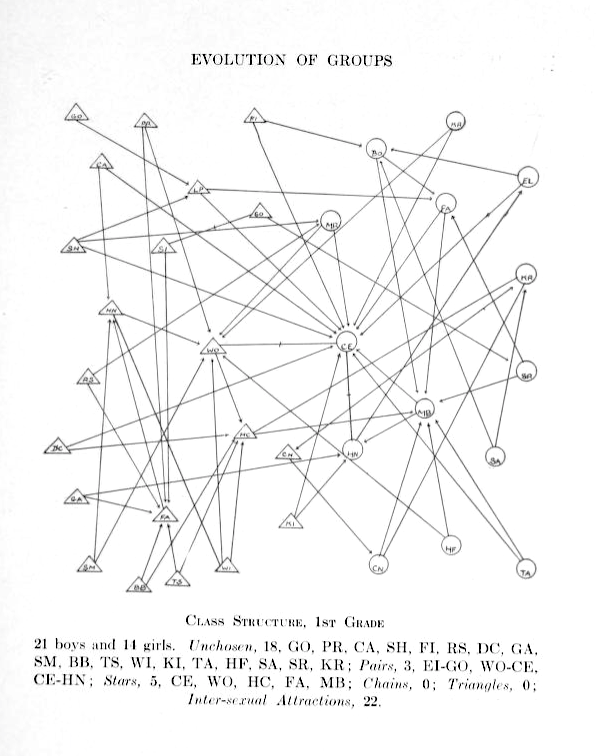
\includegraphics[width=0.4\textwidth]{static/figures/RelatedWork/Moreno-1}
    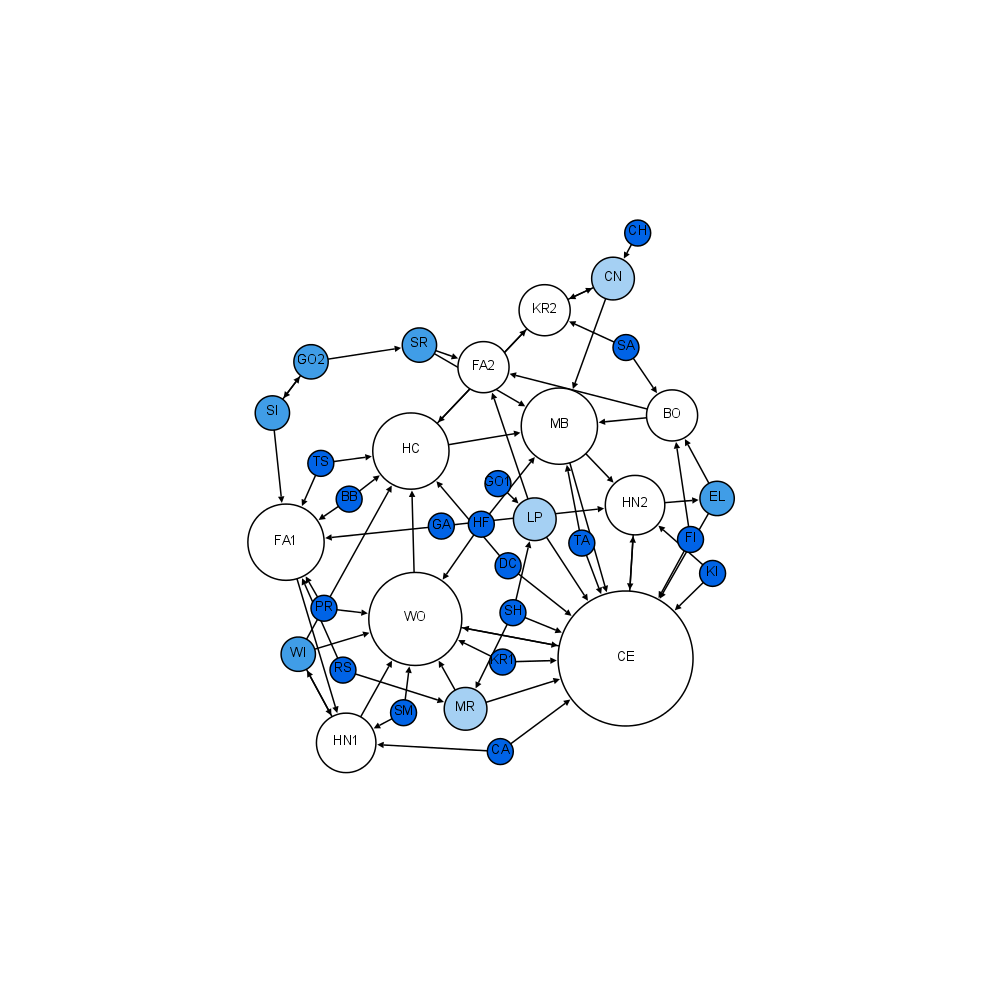
\includegraphics[width=0.55\textwidth]{static/figures/RelatedWork/Moreno-1_GrandJean}
    \caption{Moreno's original sociogram of a class of first grades from \cite{morenoWhoShallSurvive1934} (left). The diagram shows 21 boys (triangles) and 14 girls (circles). The same sociogram plot using modern practices generated from Gephi from \cite{grandjeanSocialNetworkAnalysis2015}. The color encodes the number of connections incoming.}
    \label{fig:moreno-sociogram}
\end{figure}



\subsection{Structuralism and Ego Studies}

%After SNA started to be formalized, lots of sociological studies used those concepts.
Lots of sociological studies used SNA concepts after it has been formalized.
However, there were not yet strong protocols and methods to follow, and networks are an abstraction that can model different things in different ways.
When looking retrospectively, we can see that two schools of thought emerged with different objectives and methods: the structuralists and the school of Manchester \cite{eveDeuxTraditionsAnalyse2002, maurizio2000, freemanDevelopmentSocialNetwork2004}.

%The Structural Analysis of Social Network refer to the Structuralists in Sociology.
The structuralists are interested in observing the relational structures and patterns forming a network, to make parallels between them and the social behaviors of actors in real life \cite{lazegaReseaux}.
They think the positions of the persons in the network and the relational patterns they are part of reflect well the social activities and behavior in real life.
Studying those would thus allow them to make interesting sociological conclusions.
Accordingly, sociologists in this school usually study organizations and specific groups---such as institutions, companies, families, etc.---and want to explain their functioning through the description of the internal shapes and structures of the networks.
Thus, they try to construct networks that exhaustively model all the interactions between the actors constituting the groups, as missing links would misrepresent the reality of interactions.

In contrast, the school of Manchester constituted by anthropologists focuses on studying specific individuals and all their interactions in the different facets of their lives and through time.
They typically want to explain certain behaviors and social characteristics of individuals by their relationships and interactions in all their complexity and highlight the influence of different social aspects between them in one's life.
One famous example is Mayer's study on austral Africa rural migrants going to cities \cite{mayerMigrancyStudyAfricans1962} where he showed that the integration of urban mores and customs were directly correlated to the persons' relationships networks in the city.
Xhosa\footnote{Xhosa people are an ethnic group living in South Africa and talking the Xhosa language. and studied} people still interacting with rural people of their village in the city were less changing their customs.
This school of thought typically relies on the concept of ego network and more recently dynamic and multiplex networks.
Ego networks are networks modeling all the direct relations of one central node---in this case, a person---including the relations existing between the persons of this small network.
They typically try to model the different types of relationships of a person, like their family, work, and friendship ties, and study them through time.
By studying the ego network structure of someone, sociologists of this school try to leverage explanations on other social aspects of the persons like their social status, job, and gender.
It is also common to compare several ego networks to make correlations between the social relationships of individuals and other interesting social categories.

These two methodologies of SNA are often not exclusives and current studies usually involve concepts and methods from both.
This is especially true in history where even if historians may want to describe exhaustively a group or institution of the past, they are almost always interested in specific individuals they study in depth.

\subsection{Methods and tools}\label{subsec:methods-dans-tools}

Graph theorists and network scientists developed a myriad of measures and algorithms that social scientists appropriated to describe and characterize social phenomena.
When constructing networks, the first thing sociologists do is often to identify the main actors of the network and explain why these actors are the most central, for example by linking it to their profession or social status.
Computing the degree---which is the number of connections for a node---distribution is the main straightforward way of doing it, but other more complex measures like centrality have also been developed.
Lots of types of centrality have been proposed, based on different criteria, as there are several ways of defining the more important actors.
Some centrality measures highlight actors with the highest number of connections while others highlight people bridging different groups with low interactions.
More generally sociologists aimed at identifying recurring patterns of sociability between actors.
The concepts of dyads and triads counting, which are basic structural patterns of 2 and 3 nodes, give insights into low-level relationships between people.
This reflects on Simmel's formal sociology, where he already referred to dyads and triads as a primal form of sociability \cite{Simmel2013}.
More recently, graphlet analysis extended this concept to every pattern of N-entities.
Graphlet analysis aims at enumerating every small structure of $N$ nodes composing a network, to understand how people interact at a low level.
Graphlets counting shows that graphlets are not found in a uniform distribution in social networks, thus revealing that social networks usually do not have the same structure that random networks.
This is a fact well known in SNA. Precisely, entities in real-world networks tend to agglomerate into groups (also called clusters) where entities in the same groups interact more between them than with entities from other groups.
From a sociology perspective, it means that people tend to interact and socialize in groups and interact more rarely with other people from outside groups.
These groups are often referred to as \emph{communities}, and a lot of algorithms have been proposed to find these automatically.

\section{Historical Network Research}\label{sec:historical-network-research}

If Sociology and Anthropology started to use network concepts and methods rapidly in the 1950s, it was not until the 1980s that historians started to use this type of methodology.
Yet, historians started to use quantitative methods in the 1960s, with the rise of social history, by extracting information from historical textual documents and studying them with statistical methods.
When seeing the potential of SNA concepts for historical purposes, historians started to extract the relational information contained in documents to study historical social phenomena using the power of networks and methods already developed in SNA.


\subsection{History, Social History and Methodology}\label{subsec:history-and-social-history}

History is the science of retrieving and characterizing facts about the past.
It emerged as a field with its own rules, conventions and journals in the 1880s from faculties of letters, to counterbalance previous history works which were judged as too ``literary'' \cite{noirielNaissanceMétierHistorien1990}.
History can be seen through two facets: one is societal, and serves creating a shared story for the country and a sense of unity to its citizens.
Antoine Prost says that ``it's through history than France thinks itself'' (translated from french) \cite{prost2014}.
The second facet of history constitute a methodology to describe the past in a rigorous and scientific way, with proofs.
For this, historians rely on historical documents that they leverage to infer dated facts about the past (the temporal aspects of conclusions is always central to the historian work).
The textual sources are thus at the core of the work of the historians, and having to cite historical documents and previous peers work to new claims is primordial to be considered as rigorous History work.
However, even if those two aspects are well characterized (temporal aspect of the work and its relationships to sources), methodological and epistemological facets (how historians should read and analyze their sources, how to cite them, what to report/not report etc.) of History have not been studied and discuss for a long time, until the end of the 1980s.
Some historians were interested in historiography \cite{carbonellHistoriographie1981}, but none were going to philosophical and epistemological reflexions of the History discipline.
For Lucien fèbvre, philosophising was even constituting a ``capital crime'' \cite{febvreVERSAUTREHISTOIRE1949, prost2014}.
%Les historiens font ordinairement de l’histoire sans méditer sur les limites et les conditions de l’histoire  ; sans doute, ils ont raison ; il vaut mieux que chacun fasse son métier ; d’une façon générale, il vaut mieux qu’un historien commence par faire de l’histoire sans en chercher aussi long : autrement, il n’y aurait jamais rien de fait

\alexis{maybe talk about the positivists and methodists}
At the start, history was mainly event-centered, and was focusing in characterizing central figures of the past like rulers and artists or shed light on events which shaped history like wars or political crisis.
This narrative approach to history has been criticized for its open interpretation of historical documents, which can introduce bias from the authors \cite{bourdieuRapportsEntreSociologie1995}.
%Social History emerged as a sub discipline of history with a focus on the social ascpect of history, trying to link political events (such as a revolution) to

In the 1930s, March Bloch and Lucien fèbvre detached from traditional history by creating the ``Annales school'' (Ecole des Annales) which tried to replace the human as a component of a broader sociological, political and economic system with influences between each other \cite{burkeHistorySocialTheory2005}.
They strongly advised to exhaustively search from archives, to ground historical results in documents, texts and numbers.
This new way of studying past events and societies got successful in a profession in crisis, by bringing a new lens of study on various societal subjects more grounded in the real and with a better intelligibility.
This school of thought can be seen as one of the biggest milestones for Social History, a branch of History which focuses on the socio-economical aspects of societies and their changes through time, rather than an event-centric view of History.
For example, in his thesis, Ernest Labrousse---a well known figure of Social History---tries to describe and explain the economic crisis of France at the end of the ``Ancien Régime''\footnote{The ``Ancien Régime'' is an historic period of France which starts from the beginning of the reign of the Bourbon house at 1589 until the Revolution in 1789.} through the evolution of the economic power of different social groups such as farmers, workers, property owners etc\. instead of solely describing memorable facts about the period \cite{labrousse1990crise}.
Social History continued to evolve since the 1930s, introducing new methods and concepts, but always with the goals to describe periods and historic facts through a complex and social aspect and with a strong focus on sources and traceability.



\subsection{Quantitative History}\label{subsec:quantitative-history}

%Historians try to understand an epoch using textual sources from the past, and trying to extract useful information from them.
%Social history, which is a branch of history, focus on understanding how societies were organised and how people were living together at a particular time and place. Charles Tilly argued that the task of social history lays in "(i) documenting large structural changes, (2) reconstructing the experiences of ordinary people in the course of those changes, and (3) connecting the two". For the latter, historians can leverage personal written sources---such as letters, journals, books, and newspapers---to have the internal point of view of persons living in this society and descriptions of lives of precise individuals.
%For the former, historians usually need to study more structured documents which contain information which can be extracted in a predefined and exhaustive way.
%These documents can for example be census, migration acts or marriage acts. By studying theses documents and by systematically extracting the information of these documents, historians can make global and quantitative conclusions on certain social and behavioural aspects of societies of interest.
%For example .. [EXAMPLE CHANGEMENT METIERS XXth century]

%Traditionally, historians try to tell a story about protagonists and socio-economic facts in a given society by reading, understanding, and linking together historical sources.
%This narrative approach to history has been criticized for its lack of traceability and the open interpretation of historical documents, which can introduce bias from the authors.
%To solve this problem, the ``Annales school'' (Ecole des Annales) proposed to characterize past social phenomena through the exhaustive and systematic analysis of historical documents~\cite{prost2014}.

With the development of statistical methods and more precisely Computer Science, quantitative approaches of History emerged in the 1960s with the aim of analyzing quantitative data directly extracted from historical documents.
%Using quantitative data, historians were able to make numeric conclusions on topics such as demography \cite{henryRegistresParoissiauxHistoire1956} or job distribution.
Using such methods, historians were able to make conclusions based on statistical results on topics such as demography \cite{henryRegistresParoissiauxHistoire1956} or job distribution.
For example, Gribaudi and Blum illustrated a shift in the most widespread professions in France during the 19th century using the data extracted from 50000 marriage acts \cite{gribaudi1990} and using statistical methods.

Unfortunately, quantitative and numeric methods have been criticized by historians for their simplifications and for consuming considerable time while often providing simple results \cite{karila-cohenNouvellesCuisinesHistoire2018,lepetitHistoireQuantitativeDeux1989}.
Trying to understand complex historical phenomena is complicated and modeling the information contained in historical documents into quantitative datasets can rapidly simplify and distort reality.
Moreover, quantitative historians have been criticized for focusing too much on the data, neglecting the original sources which give the context in which the data has been produced \cite{lemercierQuantitativeMethodsHumanities2019}.
Guildi and Aritage went as far as criticizing the decrease of interest of historians working in archives \cite{guldiHistoryManifesto2014}.
Approaches using digital methods and tools are nonetheless more and more popular, sometimes more recently referred to under the umbrella term Digital Humanities (DH).
If their adoption remains slow and sometimes criticized among historians, they still provide tools to store, explore, and analyze historical documents systematically if used appropriately (i.e.\ not trying to bias the analysis, and not losing the trace of the original sources).
It can also provide infrastructures and tools to study large historical databases which is more complicated to do by hand, as with the Venice Time Machine project~\cite{kaplanVeniceTimeMachine2015} which aims at digitizing and analyzing thousands of documents from the archives of Venice to understand the political, geographical, and sociological dynamics of the cities across generations and centuries.


\subsection{Historical Social Network Analysis}\label{subsec:historical-social-network-analsyis}

History started to use concepts and methods from SNA in the 1980s~\cite{wetherellHistoricalSocialNetwork1998} in order to criticize quantitative history concepts and results,
% \cite{gribaudi_categories_1990}
and to develop historical approaches---like \textit{Microstoria} \cite{ginzburgMicrohistoire1981}---that focus on the study of individuals and groups through the lens of their interactions and relationships directly extracted from historical documents.
%History started to adopt some methods and vocabulary of Network Science in the 1980s, several years after other fields such as sociology and anthropology.
Beforehand, historians were already describing and studying relational structures such as families and organizations with qualitative methods and with classical taxonomies, without studying in depth the relational aspect of these entities.
Network research allowed us to model those relational entities more thoroughly using network concepts, thus allowing us to make new observations that it was not possible to see without taking into account the relational aspects of these entities.
%Historians already had techniques and tools to annotate and extract quantitative information from textual sources that they adapted to extract and study social ties.
%We therefore saw the emergence of HNR studies, where historians studied the social relationships of actors of the past extracted from textual document and modeled into networks.
Observing and describing the structure of the resulting networks allowed historians to make conclusions on sociological aspects of the past, similar to SNA.
%followed SNA protocols on networks constructed from the mention of social ties of their textual sources.
%Using similar concepts of SNA, describing the network of social relationships of the past,
Since then, HSNA has been applied by historians to study multiple kinds of relationships, like kinship and political mobilization \cite{lippKinshipNetworksLocal2005}, administrative and economic patronage \cite{moutoukias1992}, etc.
If these approaches fall under similar critics of quantitative history \cite{lemercier12FormalNetwork2015} like the leading of trivial conclusions, it still led to classical works and interesting discoveries.
One famous example is the study of the rise of the Medici family in Florence in the 15th century by Padgett \cite{padgettRobustActionRise1993}, where he explained the rise of power of this family by their central position in the trading, marriage, and banking networks of the powerful families of Florence. \autoref{fig:padgett-medicis} shows the different networks of Florence families where we can see the central position of the Medici.
lots of historians are using and continuously improving the HSNA methods which can be very effective to study relational historical phenomena~\cite{kerschbaumerPowerNetworksProspects2015}.
Moreover, historians rarely rely on a single approach when studying an era or phenomenon, they mix methods and tools from several domains of social and formal sciences with their own practices~\cite{padgettRobustActionRise1993, petzCombiningNetworkResearch2022}.


\begin{figure}[!ht]
    \centering % avoid the use of \begin{center}...\end{center} and use \centering instead (more compact)
    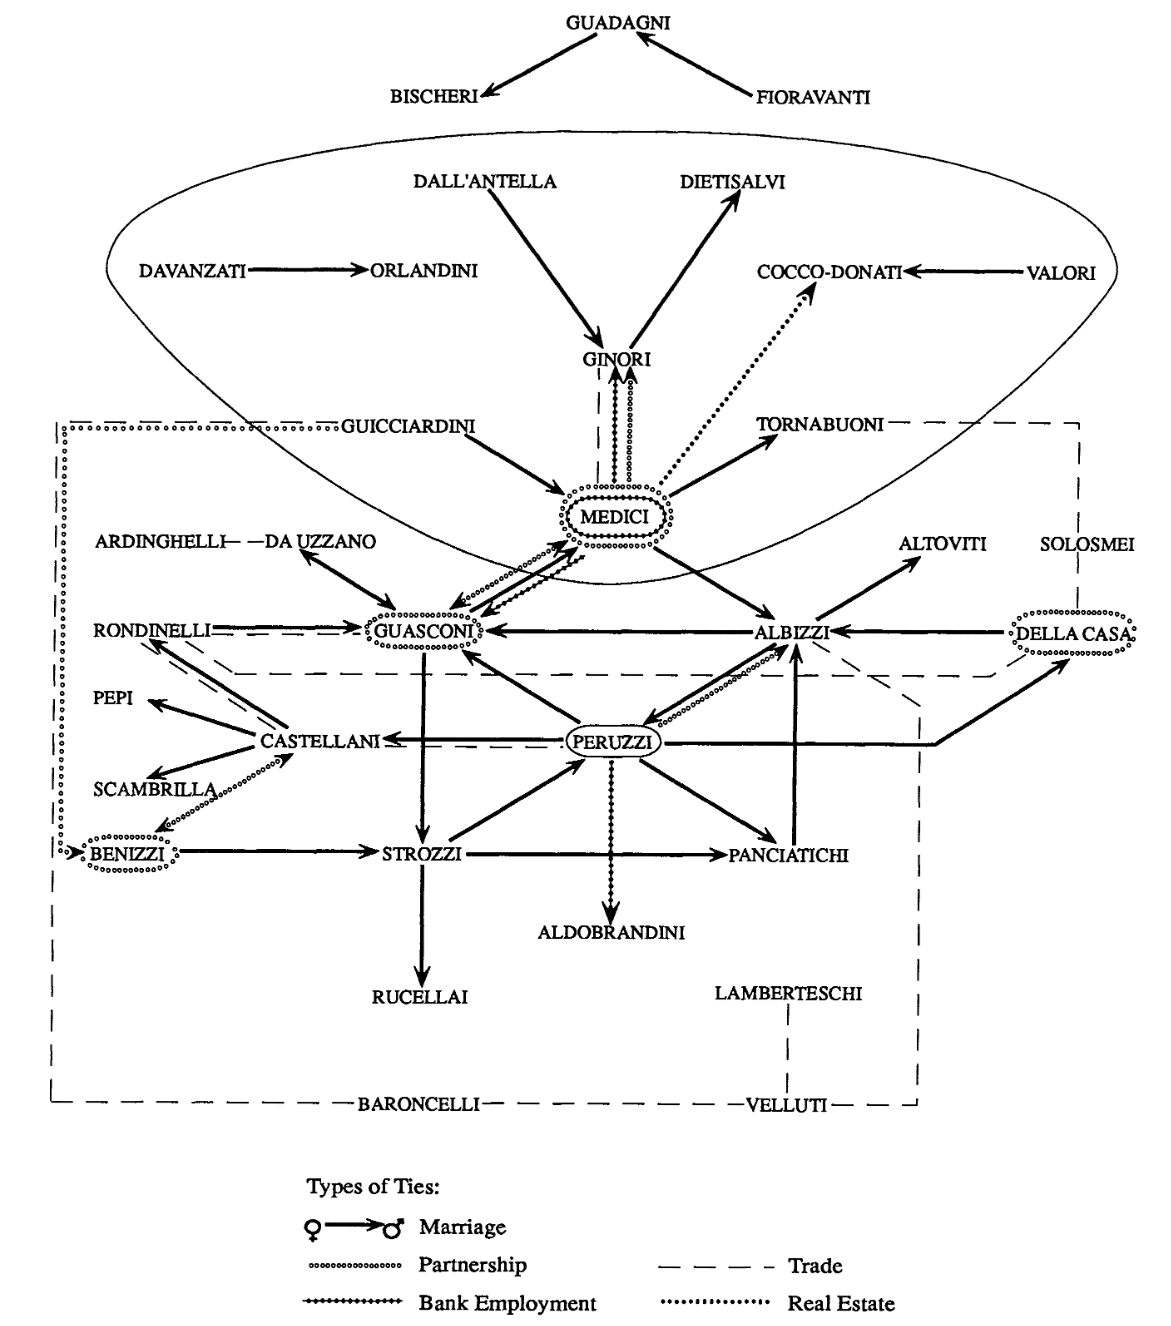
\includegraphics[width=0.8\textwidth]{static/figures/RelatedWork/padgett-Medicis.png}
    \caption{Marriage, partnership. trading, banking, and real estate networks of the powerful families of Florence from \cite{padgettRobustActionRise1993}. We can see the central position in the network of the Medici Family.}
    \label{fig:padgett-medicis}
\end{figure}

%However, constructing a network from historical sources, which can differ in their structure is not a trivial task.
%The most straightforward approach, based on the most well known social network analysis, consists in constructing social network based on simple graph $G = (V, E)$ with $V$ a set a vertices representing the persons of interest, and $E \subseteq V^2$ a set of edges modeling the social ties between pairs of persons.
%This allows to have a simple network to visualize and analyze, but does not always reflect the social complexity of the real relationships.
%More complex networks models have been proposed in SNA to be able to model more complex social relationships.


\subsection{Network Modeling}

Constructing a network from historical documents, which can vary a lot in their formats and structures, is not a trivial task.
The most straightforward and well-known approach consists in constructing a social network based on a simple graph $G = (V, E)$ with $V$ a set of vertices representing the actors of interest (very often individuals mentioned in the documents), and $E \subseteq V^2$ a set of edges modeling the social ties between pairs of actors.
This allows to have a simple network to visualize and analyze, but it does not always reflect the sociological complexity of information contained in the documents.
%More complex networks models have been proposed in SNA and HNR to be able to model more complex social relationships.
HNR network models have evolved over time to better take into account concrete properties of social networks, such as types of actors using labeled networks, the importance of actors or relations with weighted networks, mixed relationships with multiplex networks, dynamics of relations with dynamic networks.
Bipartite networks have been proposed to model relations between two types of entities, such as organization and employees where the relations link employees to organizations but not employees to employees or organizations to organizations.
Many social situations or documents can be modeled in these terms (%\textit{Interlocking directorates},
affiliation lists or co-authoring).
Multivariate networks, i.e.,  graphs, where vertices and edges can be assigned multiple ``properties'' or ``attributes'', are less used in SNA\@.
These attributes are often considered secondary, the emphasis of SNA being on the topology, its features, measures, and evolution.

Historians, demographers, sociologists, and anthropologists have also been designing specific data models for their social networks, based on genealogy or more generally kinship~\cite{hambergerKinshipNetworkAnalysis2011}.
For genealogy, the standard GEDCOM~\cite{gedcom} format models a genealogical graph as a bipartite graph with two types of vertices: individuals and families.
This format also integrates an ``event'' object but it is diversely adapted in genealogical tools.
The \href{https://www.kintip.net/}{Puck software} has extended its original genealogical graph with the concept of ``relational nodes'' to adapt the data model to more family structures and to integrate other social relationships for anthropology and historical studies~\cite{hambergerScanningPatternsRelationship2014}.


\section{Social Network Visualization}\label{sec:social-network-visualization}

Practitioners of SNA and HSNA have always depicted visually their networks for validation and communication purposes, mostly using node-link diagrams.
With the increase in average network size and the diversity of network models, new visualization techniques have been proposed to represent the diversity of studied networks.
Moreover, more and more social scientists are following exploratory approaches using Visual Analytics (VA) tools, to describe more in-depth their data and generate new interesting hypotheses, using interaction and exploration capabilities.

\subsection{Visualization}

Data Visualization consists in graphically displaying data for the purpose of enhancing human cognition capabilities to understand and communicate ideas and phenomena.
History is filled with classical examples of visual data displays which helped understand real phenomena, such as Minard's map of Napoleon's march in Russia \cite{friendlyVisionsReVisionsCharles2002}, or Snow's dot map of cholera cases in London which showed the proximity between street pumps and cholera infections \cite{snowModeCommunicationCholera1856}.
If several examples of data visualization can be found thorough history, it mainly developed as a scientific field in the 1960s with Tukey's work on data analysis and visualization \cite{tukeyFutureDataAnalysis1962} and Bertin's publication of Semiology of graphics \cite{bertin1967}.
In this foundational work, Bertin described and organized the different visual elements usable in graphical information displays, and linked them to data features and relations types.
Friendly says ``To some, this appeared to do for graphics what Mendeleev had done for the organization of the chemical elements'' \cite{friendlyBriefHistoryData2008}.
The development of computer science and the rise of hardware capabilities during the same time created a big need for data visualization.
The amount of data stored increased exponentially and descriptive statistics were not enough to understand the underlying structure of the amount and diversity of produced data.
Visualization, leveraging the human visual system, allows to rapidly see the hidden structure of a dataset and detect interesting and unexpected patterns very often unseen with classical statistical methods.
One classical illustration of this is Anscombe's quartet \cite{anscombeGraphsStatisticalAnalysis1973} which consists of four datasets of points in $\mathbb{R} ^{2}$ with the same statistical measures (mean, variance, correlation coefficient, etc.) but with very different structures, that plotting the data show immediately.
The four datasets are illustrated in \autoref{fig:anscombe-quartet}.


\begin{figure}
    \centering % avoid the use of \begin{center}...\end{center} and use \centering instead (more compact)
    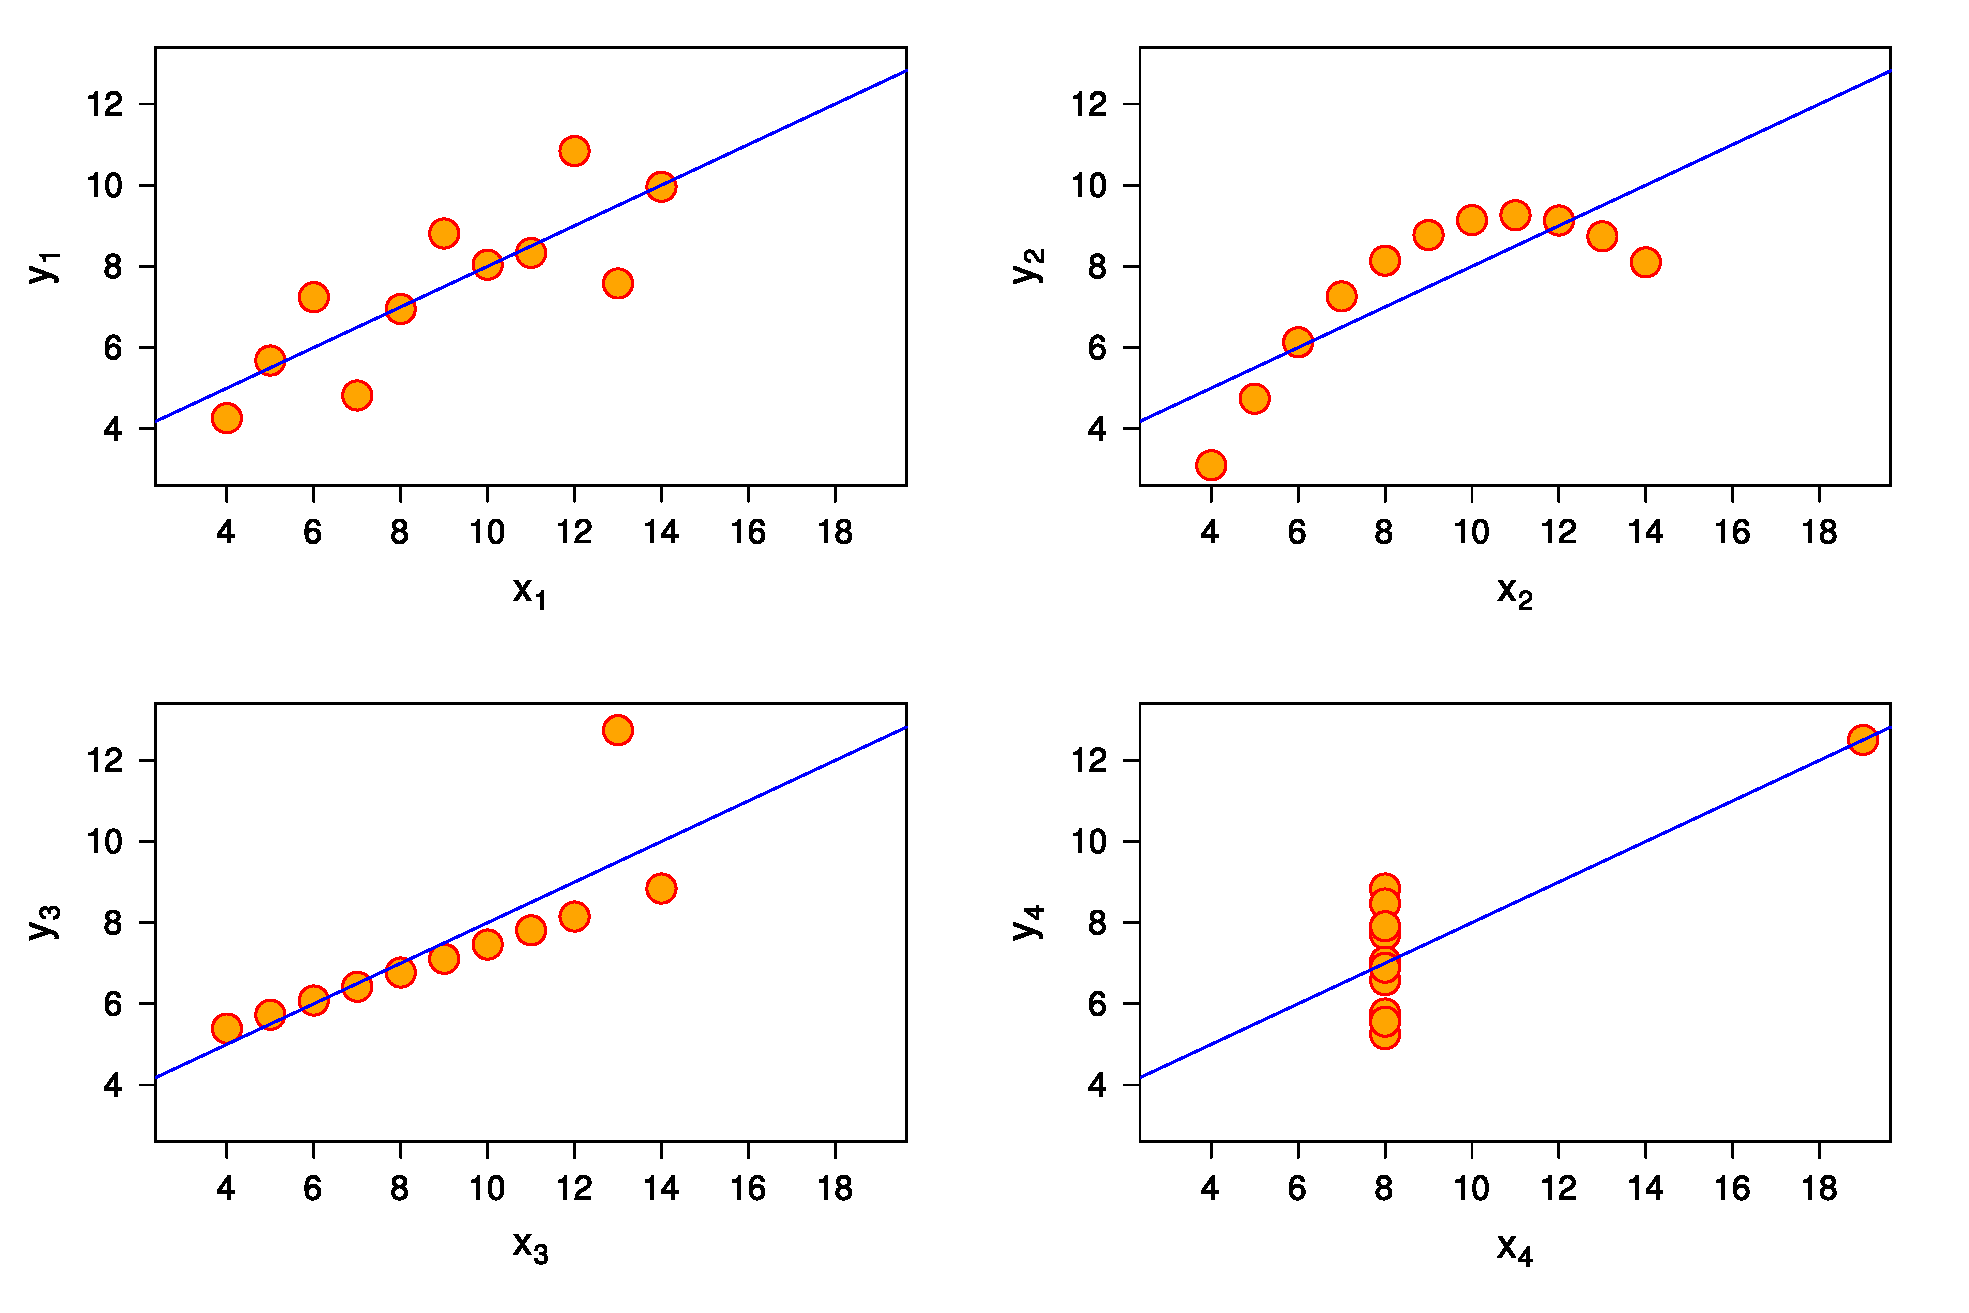
\includegraphics[width=0.8\textwidth]{static/figures/RelatedWork/Anscombe.pdf}
    \caption{Anscombe quartet. The four datasets have the same descriptive statistics (average, variance, correlation coefficient) but very different structures. Image from \cite{anscombeGraphsStatisticalAnalysis1973}.}
    \label{fig:anscombe-quartet}
\end{figure}


Lots of visualization techniques emerged to make sense of the diversity of data produced, such as relational, temporal, spatial, or network data.
Subfields of Visualization emerged: \textbf{Scientific visualization} focus on visualizing continuous real data such as weather, spatial, and physics data, sometimes produced with simulations whereas \textbf{Information Visualization} is centered around the visualization of (multidimensional) discrete data points, often in an abstract way. \textbf{Visual Analytics} emerged later from Information Visualization by mixing data mining and more complex analysis process with traditional information visualization displays.
Historical Social Network visualization is closely related to Information Visualization and Visual Analytics, and good visualization systems for HNR use concepts and methodologies from those two fields.

%Grammar of graphics

\subsection{Social Network Visualization}

Sociologists rapidly saw the potential of graphically showing relationships between individuals, to better comprehend the underlying social structure and communicate their findings.
Moreno elaborated sociograms to visually show friendships among schoolchildren with circles and lines to respectively show children and friendships ties \cite{morenoWhoShallSurvive1934}.
This type of representation---commonly called node-link diagram---is the most widely used in social sciences, as it is rapidly understandable and effective for small to medium-sized networks which is usually the norm in social sciences.
The most used social network visual analytics software such as Gephi \cite{Gephi} and Pajek \cite{mrvarAnalysisVisualizationLarge2016} are based on this type of representation and allow a fully integrated exploration and analysis with the help of various algorithms.
Finding an optimal placement for the nodes is however not that simple as several metrics can be optimized depending on the desired drawing, such as the number of edge crossings, the variance of edge length, orthogonality of edges, etc~\cite{cristofoliPrincipesUsagesDessins, kosakAutomatingLayoutNetwork1994}. \autoref{fig:kosak-graph-drawing} shows some of these metrics, synthesized by Kosara and al.~\cite{kosakAutomatingLayoutNetwork1994}.
In \autoref{fig:moreno-sociogram} we can see the difference in readability between the original manual layout (left) and an automatic one (right).
Automatic layouts which aim at optimizing readability metrics give clearer diagrams.
The number of edge crossings is often considered the most important measure, but finding a drawing with the optimal number of crossings is an NP-Hard problem, meaning that heuristics are needed for most real-world use cases.
Lots of algorithms have been designed such as force-directed ones, modeling the nodes as particles that repulse each other and are attracted together when connected with a link that can be seen as strings.
Other visual techniques have been proposed to represent networks such as matrices, circular layouts, and arcs, but are less used in social sciences \cite{mcguffinSimpleAlgorithmsNetwork2012}.
Still, Matrices have been shown to be better than node-link diagrams for a lot of tasks such as finding cluster-related patterns, especially for medium to large networks \cite{ghoniemComparisonReadabilityGraphs2004}.

\begin{figure}
    \centering % avoid the use of \begin{center}...\end{center} and use \centering instead (more compact)
    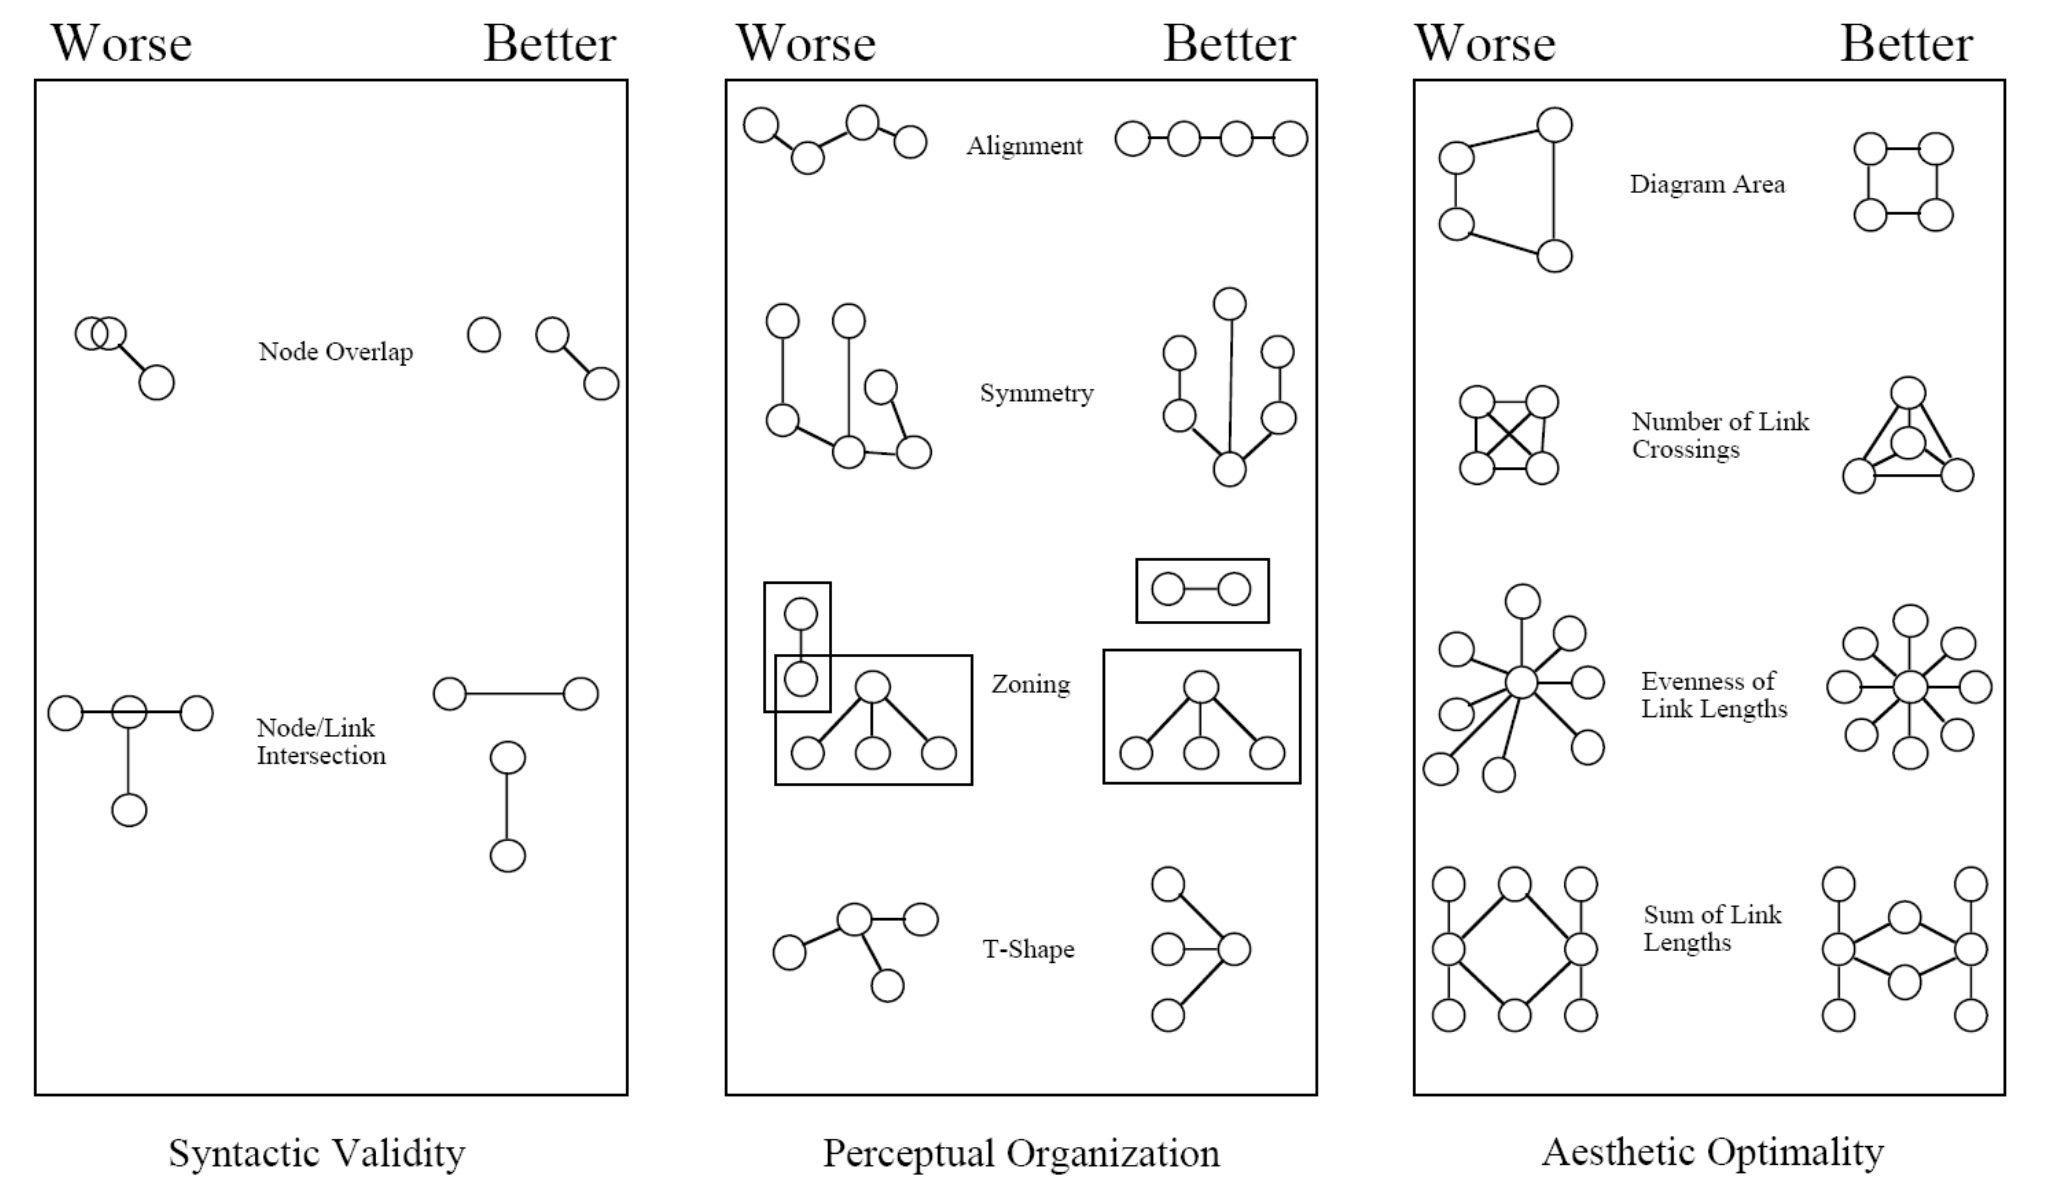
\includegraphics[width=1\textwidth]{static/figures/RelatedWork/Kosak-nodelinkdiagramMetrics}
    \caption{Different criteria are proposed to enhance node-link diagram readability. Image from \cite{kosakAutomatingLayoutNetwork1994}}
    \label{fig:kosak-graph-drawing}
\end{figure}

As social scientists started to use more complex network models such as bipartite or temporal networks, more sophisticated representations are needed.
%The visualization community proposed new visualization systems for specific network types such as PAOHVis for temporal hypergraphs, NodeTrix for clustered networks or Juniper for Multivariate networks.
The visualization community developed new representations to visualize other network types such as dynamic hypergraphs with PAOHVis \cite{valdiviaAnalyzingDynamicHypergraphs2021}, clustered graphs with NodeTrix \cite{henryNodeTrixHybridVisualization2007} (illustrated in \autoref{fig:Riche-NodeTrix}), geolocated social networks with the Vistorian \cite{serranomolineroUnderstandingUseVistorian2017}, and multivariate networks with Juniper \cite{nobreJuniperTreeTable2019}.
However, these new network representations take time to be adopted by social scientists who rarely use those.


\begin{figure}
    \centering % avoid the use of \begin{center}...\end{center} and use \centering instead (more compact)
    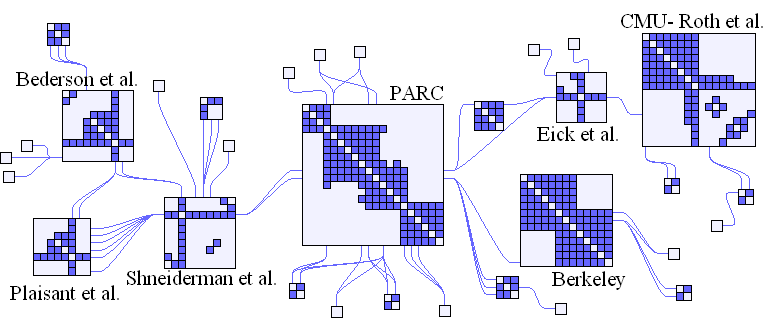
\includegraphics[width=0.8\textwidth]{static/figures/RelatedWork/NodeTrix.png}
    \caption{NodeTrix system showing a scientific collaboration social network with clusters. Each cluster is represented as a matrix,  Image from \cite{henryNodeTrixHybridVisualization2007}.}
    \label{fig:Riche-NodeTrix}
\end{figure}


\subsection{Social Network Visual Analytics}

Social network visualization has mostly been used for confirmatory and communication purposes from its beginning.
Social scientists often had hypotheses that they could rapidly verify by plotting the data.
The same plots were often used for communication purposes, for example in a scientific paper or presentation.
However, visualization can also be used for exploratory aims, to gain new insights into the data and potentially generate new hypotheses.
This process has been characterized by Tukey in 1960 as \emph{Exploratory Data Analysis (EDA)}.
Exploration is mostly possible thanks to interaction, which allows changing the point of focus in the data to highlight interesting patterns, with the help of mechanisms like filtering, querying, sorting, etc.
As the average size of datasets keeps growing, exploratory tools are often needed to make sense of large datasets and generate interesting hypotheses.

Social scientists also often want to gain insight with the help of statistical and machine learning methods, that visualization only can not provide.
More recent visual exploration interfaces incorporate automatic analytical tools along with graphical displays, letting users apply data mining algorithms directly in the exploratory loop.
This coupling of visualization and data mining has been defined as Visual Analytics (VA) and is still undergoing lots of research.
Keim and al.\ define it as ``a combination of automatic and visual analysis methods with a tight coupling through human interaction in order to gain knowledge from data'' \cite{keimVisualAnalyticsDefinition2008}. \autoref{fig:keim-va} shows an abstract representation of the VA process.

\begin{figure}
    \centering % avoid the use of \begin{center}...\end{center} and use \centering instead (more compact)
    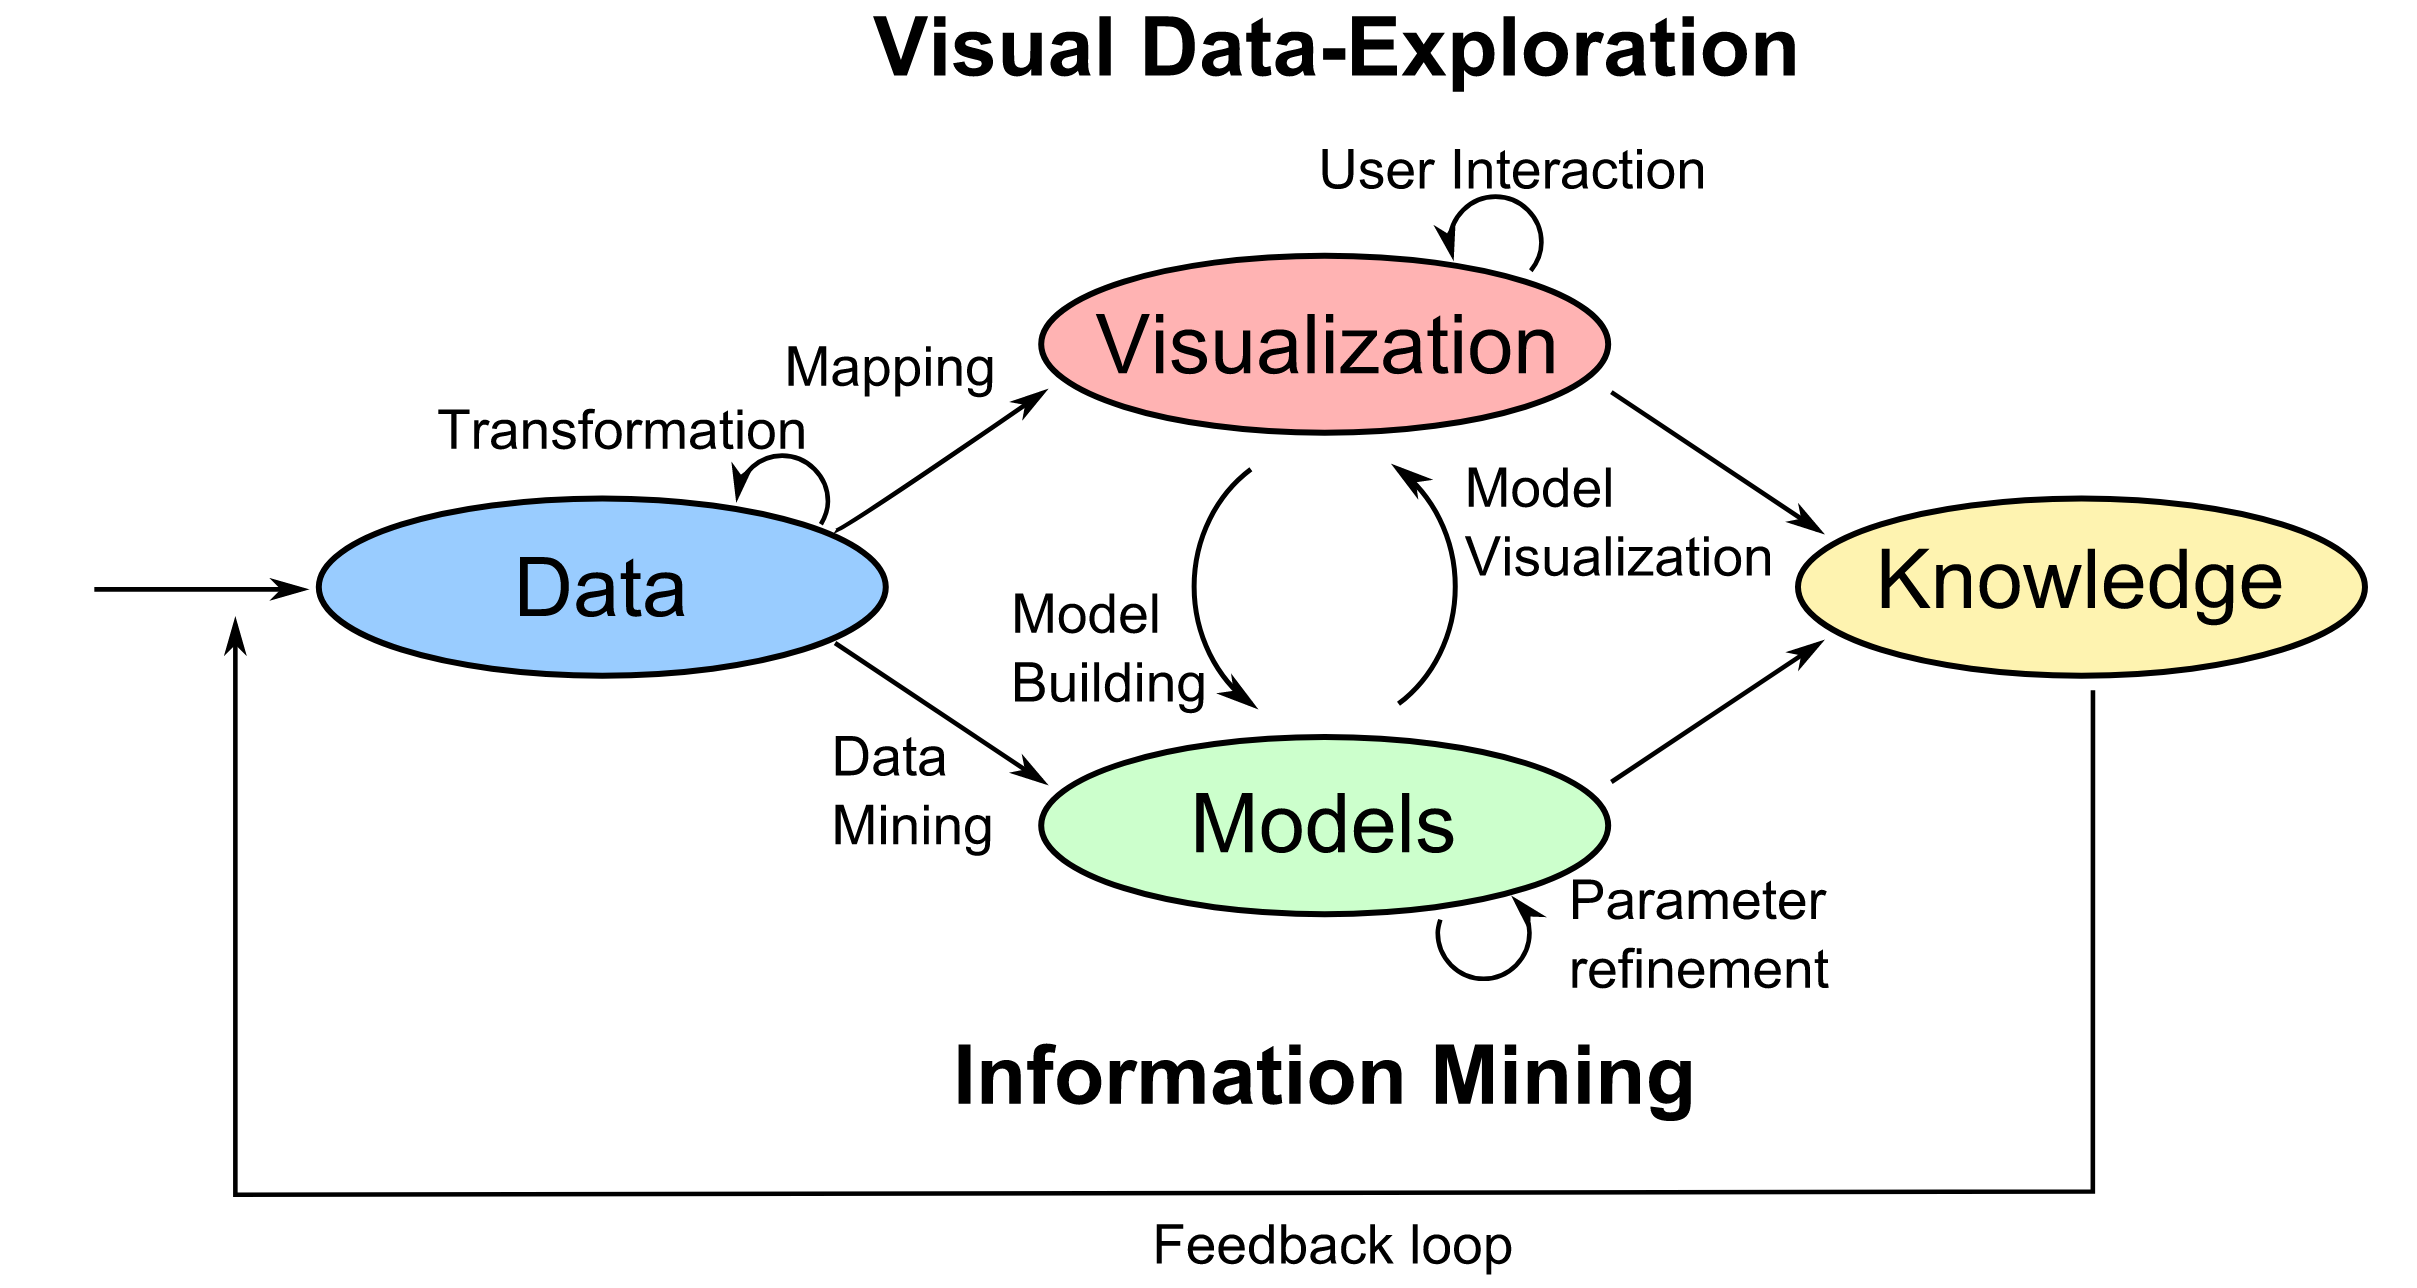
\includegraphics[width=1\textwidth]{static/figures/RelatedWork/Keim-VisualAnalytics.png}
    \caption{Abstraction of the VA process. It is characterized by continuous interactions between the data, visualizations, models, and knowledge. Image from \cite{keimVisualAnalyticsDefinition2008}.}
    \label{fig:keim-va}
\end{figure}

It is defined around the generation of knowledge using visualizations and models of the data, that the user generates and explores using interaction.
Social scientists now frequently use VA systems to make sense of their data by using visualization, interaction, and data mining algorithms in their analysis loop to find interesting patterns and verify and create hypotheses.
The most used social network VA tools are Gephi \cite{Gephi}, Pajek \cite{mrvarAnalysisVisualizationLarge2016}, and NodeXl \cite{NodeXL}. \autoref{fig:gephi} presents the Gephi interface showing a clustered social network, where each node is part of a cluster, encoded by color.
They all let users visualize their networks with a node-link diagram, and allow an interactive exploration of the data with operations like filtering.
Users can also analyze their data using network measures computed directly in the interface, and apply data mining algorithms such as clustering which results are explorable visually.



\begin{figure}
    \centering % avoid the use of \begin{center}...\end{center} and use \centering instead (more compact)
    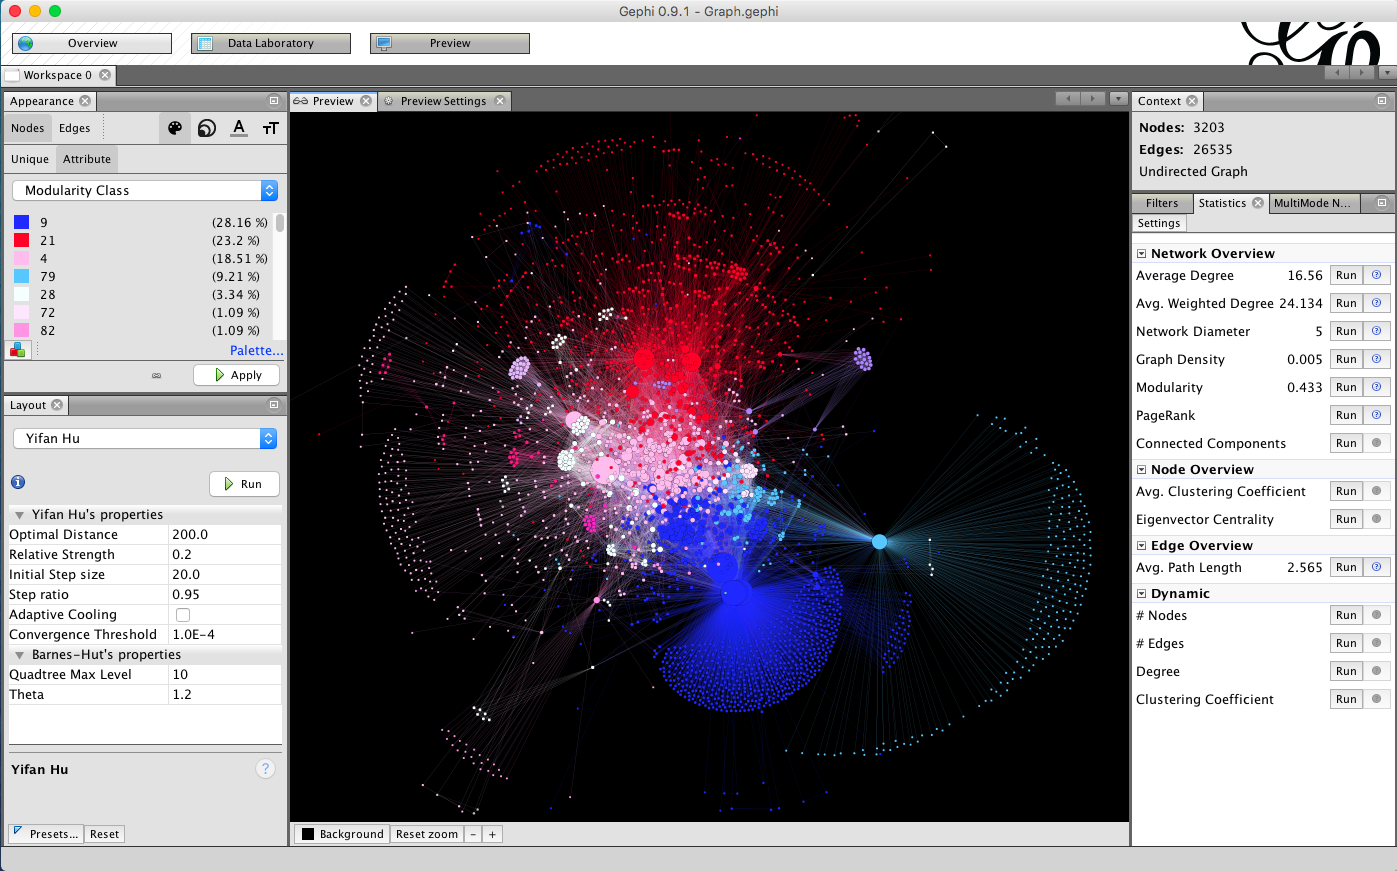
\includegraphics[width=0.8\textwidth]{static/figures/RelatedWork/Gephi_0.9.1_Network_Analysis_and_Visualization_Software}
    \caption{Gephi \cite{Gephi} interface. The network is represented with a node-link diagram. Users can interact on the visualization and encode node and links visual attribute (color, size etc.) with network measures computed directly in the interface, such as the node degree, or clustering results.}
    \label{fig:gephi}
\end{figure}

Unfortunately, social scientists are often not trained in computer science and mathematical methods, and a lot of them have been frustrated by VA tools and by how it was guiding their analysis in predefined ways.
For example, lots of social network VA interfaces propose clustering features, allowing users to find interesting groups with the help of automatic algorithms, but social scientists often do not understand how the algorithms work and are not always satisfied with the results, as they can have knowledge from other sources not modeled inside the network.
They usually end up trying several algorithms until they stumble upon a satisfactory enough solution.
Cleaning and importing the data is also complicated, as the annotation and network modeling process are not straightforward and social scientists often encounter errors and inconsistencies in the data once they visualize it, that they would like to correct.
Historians thus always have to go back and forth between their analysis process inside the VA tool they are using, and their original sources and annotation/modeling process, to correct errors or modify annotations.
Interestingly, the chosen network model plays a big role in this process, as a simple network model representing only the persons (as it is often the case) will make it harder to trace back to the original documents containing the annotations from the network entities.
Yet the majority of Social Network VA interfaces enforce simple network models, making this retroactive process harder.
Some interfaces still incorporate data models encapsulating document representations, such as Jigsaw \cite{staskoJigsawSupportingInvestigative2008} which allows an exploration of textual documents with their mentioned entities.
Finally, more work is still to be done on social network VA tools, to provide more guidance and power to social scientists while doing their analysis, and to help them to do easier back and forth between their analysis and the annotation, network modeling, and cleaning steps, as they play a big role in the historian workflow.



